\documentclass{report}


\usepackage[ngerman]{babel}
\usepackage[utf8]{inputenc}
\usepackage[T1]{fontenc}
\usepackage{hyperref}
\usepackage{csquotes}
\usepackage[a4paper]{geometry}

\usepackage{graphicx}
\usepackage{float}
\usepackage{caption}

\usepackage[
    backend=biber,
    style=apa,
    sortlocale=de_DE,
    natbib=true,
    url=false,
    doi=false,
    sortcites=true,
    sorting=nyt,
    isbn=false,
    hyperref=true,
    backref=false,
    giveninits=false,
    eprint=false]{biblatex}
\addbibresource{../references/bibliography.bib}


\title{Ethik im Umgang mit Daten}
\author{Levin Kaya}
\date{\today}



\begin{document}

% Hier wird die Titelseite gestaltet.
\begin{titlepage}
    \makeatletter % Das hier brauchen wir damit wir spezielle Befehle wie \@author verwenden können.
	\begin{center}
		{\scshape Gymnasium Muttenz} \vspace{0.5cm}
        
        Informatik 2023/2024\vspace{5.5cm}
        
		{\huge\bfseries \@title}
        
		\vspace{2cm}
        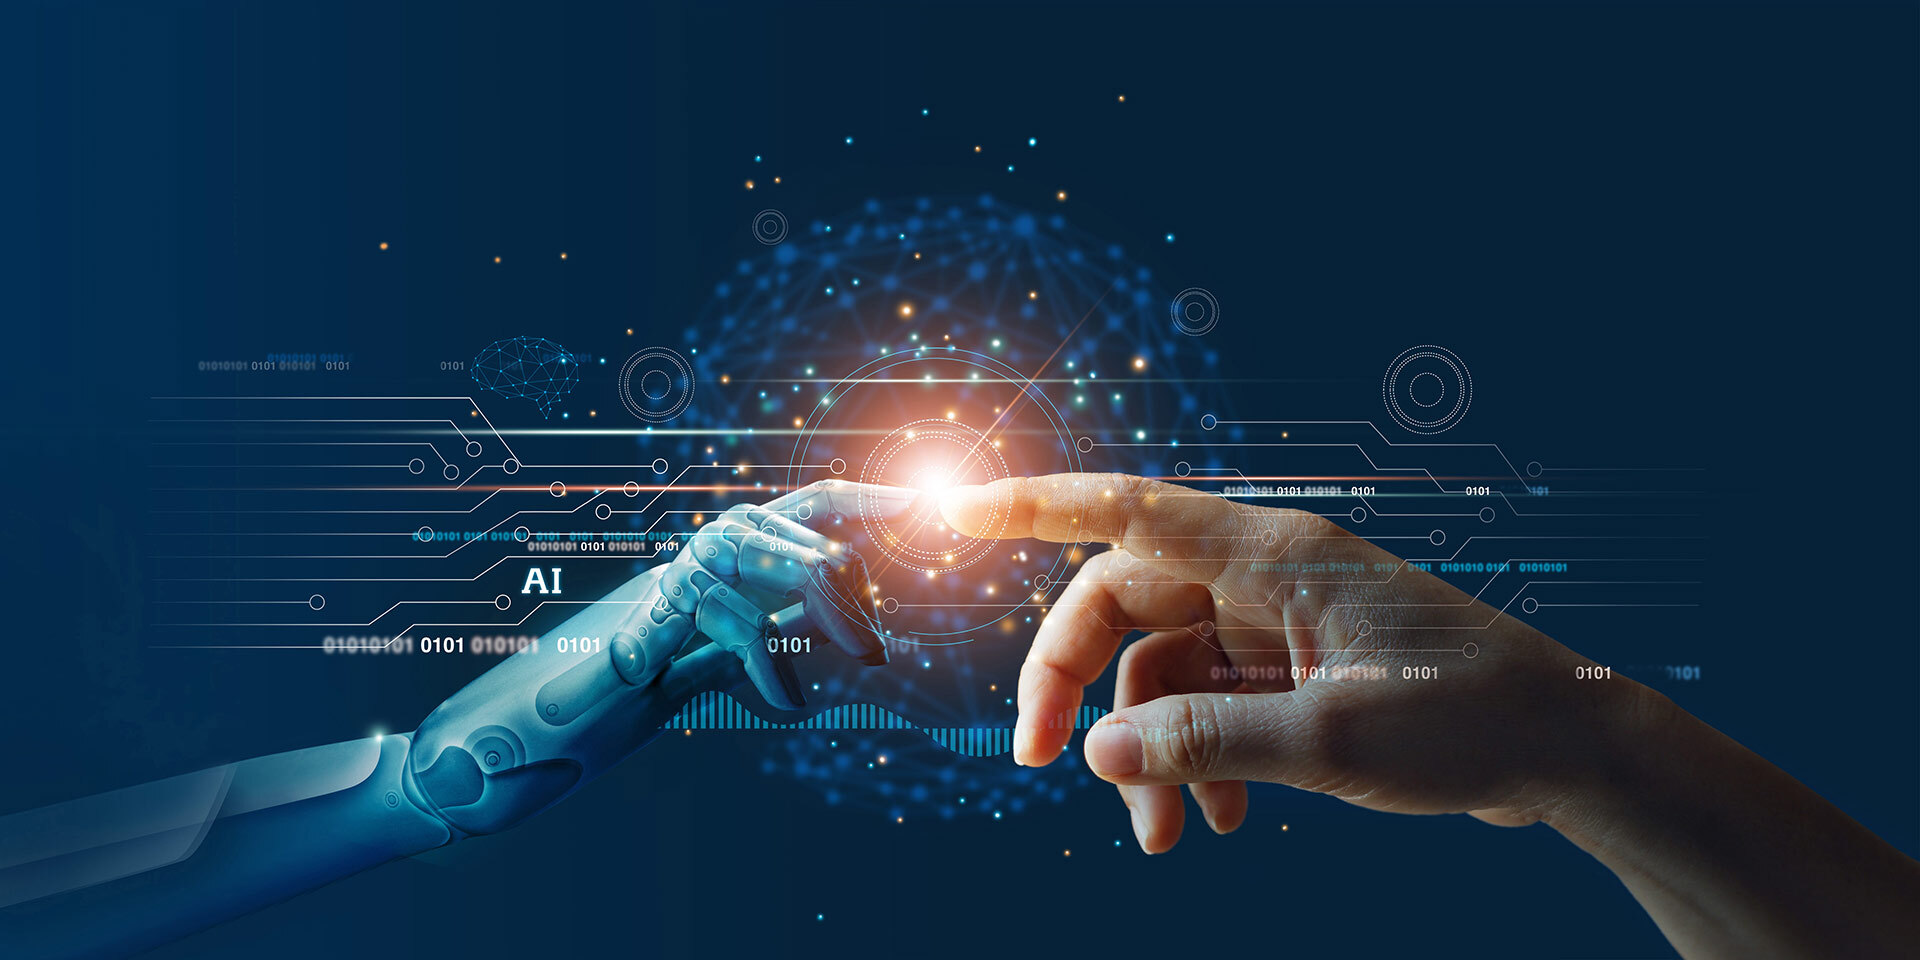
\includegraphics[width=0.5\textwidth]{KI.jpg}

		\vspace{2cm}

		{\Large\itshape \@author}

        \vspace{2cm}

        Version vom: \@date
	\end{center}
    
    \makeatother % Wir müssen das @ wieder schliessen, damit der Rest ganz normal funktioniert.
\end{titlepage}

\abstract{
    In folgendem Aufsatz werde ich zu meiner selbst gewählten Fragestellung Bezug nehmen und dabei die verschiedenen Aspekte der KI, sowie deren Auswirkungen und Problematiken analysieren und versuchen näher zu bringen.






}

\tableofcontents

\chapter{Einleitung}



\section{Einleitung}
Zu Beginn dieser Arbeit werde ich auf die allgemeine Frage, woher die KI ihre Informationen bezieht eingehen und um welche spezifischen Datenquellen es sich dabei handelt. 
\subsection{Datenfütterung}
Das sogenannten Large Language Modell (LLM) wird von einer gigantischen Menge an Informationen aus dem Internet gefüttert, darunter milliarden von Büchern, Artikeln, Websites und Posts.
\subsection{Filterung der Quellen} 
Die Qualität der Informationen variiert dabei extrem, von seriösen, vertraulichen Quellen wie beispielsweise wissenschaftlicher Lieratur bis hin zu völlig falschen Angaben aus Foren oder sozialen Medien. Aus diesem Grund werden einige unerwünschte Inhalte, wie ''Wie baut man eine Bombe'' herausgefiltert und nicht beantwortet. Während dieses Prozesses werden zudem doppelte Quellen, sogennante Duplikate gelöscht. Die gesammelten Daten werden bereinigt und in ein Format gebracht, das das Modell verarbeiten kann.
\subsection{Das Trainieren der KI} 
Genau auf diese Art und Weise wird also Chat GBT trainiert, sie ist nämlich ein Modell, bei welchem Einträge gemacht werden, so lange, bis sie präzise werden und ziemlich wahrscheinlich der Wahrheit entsprechen. Kleine Abschnitte werden durch viele Schichten dieses Modelles geschickt. Wenn also immer wieder Einträge gemacht werden, kann es so trainiert werden, dass die Antworten, die die KI generiert aus vielen unterschiedlichen basieren und somit immer effizienter und genauer werden. Nutzerinnen und Nutzers können mit einem ChatBot kommunizieren und eine Eingabe erstellen wie z.B. ''Wie verbessere ich meinen Schlaf?'' Nach dem Begriff durchsucht der Bot das Netzwerk und kombiniert dies mit der Eingabe. Er sucht den Begriff ''Schlaf'' und versucht diesen mit der Eingabe in einen Kontext zu bringen. Seine Rückgabe ist demnach eine Berechnung der Wörter, die am ehesten darauf folgen. Im gewählten Beispiel ''Wie verbessere ich meinen Schlaf'' antwortet die KI vermutlich mit ''regelmässige Schlafzeiten'' als vorhersehbarste Lösung. Die Qualität der Vorhersagen, welche die KI als Lösung zurückgibt werden dadurch berechnet,wie weit die Vorhersagen vom tatsächlichen nächsten Wort entfernt sind.
Die Gewichte, die Parameter genannt werden durch Optimierungsalgorhytmen angepasst. Das Ziel des Trainierens ist es, über viele Schritte hinweg die Fehler der künstlichen Intelligenz zu reduzieren. Die Gewichtung der Parameter sind ausschlaggebend für das Modell.

\subsection{Das Validieren und Testen}
Durchs Validieren kann man beim KI- Modell sicherstellen, dass es sich bei den Rückgaben nichz ausschliesslich um auswenig gelernte Inhalte handelt, sondern dass sie das Muster versteht. Das Ziel ist es, dass es möglichst gut in der Lage ist, auf ähnliche Fragen, auf die es nicht direkt trainiert wurde zu antworten. Die Ersteller hinter dem Ganzen wollen ein Sprachmodell erstellen, welches leistungsfähig und facettenreich ist. Selbst nachdem das Modell vollständig ist wird es auf einem sogenannten seperratem ''Testdatensatz'' geprüft.


\section{Fragestellung}
Kann man sicherstellen, dass die Antworten, die von einer Künstlichen Intelligenz generiert werden, auf vertrauenswürdigen und nachvollziehbaren Quellen basieren, welche ethischen Werte vertritt es und welche Problematiken gehen damit einher?

\section{Die Problematik der Quellenverwendung und -genauigkeit bei Künstlicher Intelligenz, sowie ethische Herausforderungen}

Wie bereits in meiner Einleitung beschrieben und in meiner Fragestellung erläutert, werde ich nun explizieter auf die Informationsquellen der KI und der mit sich bringenden Problematiken eingehen. Das Trainieren der KI habe ich bereits erklärt und ebenfalls das es auf die Korrektheit der Quellen keine Garantie gibt. Es gibt jedoch eine weitere Problematik, nämlich der Fakt das die KI- Informationen aus dem Internet extrahiert. Weil der Chatbot sich die Arbeit zu eigen macht, ohne die Urbheber zu entlohnen oder zu nennen, handelt  es sich um ein Raub der Quellen. Zudem veröffentlicht das kalifornische Unternehmen ''Open AI'', das hinter beispielsweise ChatGBT steckt nicht die explizieten Trainingsdaten, die benutzt werden um die KI zu trainieren und es ist auch weiterhin sehr unklar wie der genaue Verlauf der Weiterverarbeitung der Informationen aus dem Netz verläuft. Häufig stellt man auch fest, dass wenn man ChatGBT beispielsweise über aktuellere Tatsachen fragt, es keine so spezifischen Antworten geben kann. Dies ist darauf zurückzuführen, dass es nur mit Daten bis 2021 gefüttert wurde. Eine weitere Problematik, auf die ich eingehen möchte ist die Tatsache, dass es sehr gefährlich ist, ChatGBT für Bildungs- und Weiterbildungszwecke zu verwendenden, da Falschinformationen weitergegeben werden können. Vorallem bei Primar- und Sekundarschulstoff Inhalten, sollte komplett auf KI verzichtet werden. 
Bei Chatsbots wie ChatGBT kommt es desöfteren vor, dass falsche oder verwirrende Ausgaben gegeben werden. Bei kleinen Kindern ist es nicht auszuschliessen, dass sie diese Informationen glauben könnten, da sie noch nicht wissen, wie man Informationen kritisch hinterfragt und überprüft. Um zu vermeiden, dass Grundschulkinder diese Falschinformationen in der Schule oder Zuhause verwenden und dadurch falsche Vorstellungen entwickeln, ist es wichtig das man auf die menschlichen Kompetenzen der Lehrkräfte zählen kann und dass diese keine Chatbots mit nicht zurückverfolgbaren Quellen verwenden. In folgender Auflistung habe ich die negativen Aspekte, welche Problematiken hinter der KI darstellen grob aufgelistet, als Übersicht zum Fliesstext.
\section{Problematiken der KI}

\begin{itemize}
 
    \item Falschinformationen
    \item Verständnisprobleme
    \item Fehlende Transparenz
    \item Urheberechtsverletzung
    \item Ethik
    \item  Verlass auf KI, anstatt eigenständigem Lernen
 
\end{itemize}

\section{Fazit}
In meinem Fazit zur Fragestellung, ob man sicherstellen kann, dass die Antworten, die von einer Künstlichen Intelligenz generiert werden, auf vertrauenswürdigen und nachvollziehbaren Quellen basieren, welche ethischen Werte sie vertritt und welche Problematiken damit einhergehen, werde ich die wesentlichen Punkte zusammenfassen und werde erläutern, was man als Schlussfolgerung aus meiner Arbeit ziehen kann. Schlussendlich können wir, als Nutzer der KI nicht wissen, ob es sich bei den gegeben Informationen wirklich um die Wahrheit handelt oder es nicht auch sein könnte, dass diese so manipuliert wurden, dass uns die Informationen weitergegeben oder vorenthalten werden, die die Ersteller selbst vertreten. Die ethischen Werte, die die KI vertritt, sind eng mit den der Entwickler und der betreibenden Organisation (Open AI) verknüpft. Da diese Werte  nicht immer offengelegt werden und grösstenteils untransparent bleiben, bleibt unklar, inwieweit die KI ethische Grundsätze wie Fairness, Transparenz und Verantwortlichkeit einhält. Dies ist auch einfach für Nutzer zu beobachten, da ChatGBT auf moralische Fragen meist uneindeutige Ausgaben gibt. Dies kann grosse Folgen haben im Bereich der Bildung. Schlussendlich kann man derzeit nicht mit absoluter Sicherheit davon ausgehen, dass Antworten, die KI- generiert sind auf 100 Prozent vertrauenswürdigen und nachvollziehbaren Quellen basieren. Dadurchs entsteht eine grosse Unsicherheit, was das Vertrauen an ChatGBT angeht, denn wie nun mehrmals erklärt handelt es sich hierbei um viel Intransparenz bei den Datenquellen und ethischen Richtlinien. Meiner Meinung nach dient ChatGBT gut dazu, wenn man sich Allgemein Hilfe sucht wie beispielsweise beim kürzen von Texten, wenn man eine Idee sucht ( zb. im kreativen Bereich ), bei Analysen und auch sehr bei Sprachkenntnissen und grammatikalischen Fragen. Jedoch sollte dem Nutzer/ der Nutzerin auch klar sein, dass bei Arbeiten, bei denen seriöse Quellen erwartet werden, nicht auf ChatGBT zurückgegriffen werden kann. Daher ist ausschlaggebend, dass vorallem was den Bereich des Bildungswesen angeht, menschliche Kompetenzen und Fachwissen genutzt werden sollten, um sicherzugehen das ethische Grundsätze und das Verbreiten von falschen Informationen streng kontrolliert werden.
 
\nocite{*}
\printbibliography

\end{document}
